\chapter{Implementácia}

\todo daky pokec o tom ze som to pisal v pythone a preco je python super

\section{Použité knižnice}

\subsection{Realigner}
\todo cosi k micovmu kodu - mozno referencia na jeho dizertacku + mozno nejaky pokec k tomu ze co sme pouzili a mozno ako to funguje

\subsection{Pyhonové knižnice}
\todo python kniznice - najma scikit-learn, numpy, track

\section{Triedy na zarovnávanie s klasifikátorom}

\subsection{Predspracovanie dát}

\todo DataPreparers, class diagram

\subsection{Zovšeobecnenie klasifikátora}

\todo PairClassifier

\subsection{HMM stavy s klasifikátorom}

\todo Classifier state...

\section{Pomocné programy}
\subsection{Simulátor}

Simulátor sĺuži na overenie funkčnosti zarovnávača. Náhodne vygeneruje 2 sekvencie, ktoré vznikli zo spoločného predka a vyrobí korektné zarovnanie. Okrem toho vyrobí aj nejaké dodatočné informácie ktoré majú pomôcť pri zarovnávaní.

\subsubsection{Algoritmus}
Simulátor vygeneruje informáciu o tom, ktoré časti sekvencie prisĺuchaju génom a ktoré nie. Informácia má podobu boolovskeho vektora.
Simulátor najskôr vygeneruje \textit{základnú (master) postupnosť} a z nej odvodí dve ďalšie postupnosti, ktoré zodpovedajú sekvenciám.

Okrem toho simulátor vygeneruje dve sekvencie, pričom prvú vyrobí náhodne a druhú odvodí z nej pomocou mutácie a inzercie/delécie.
V našom prípade sme inzerciu vynechali a simulujeme ju ako deléciu v druhej sekvencii.
Pri odvodzovaní bude používať aj informáciu o tom, ktorá časť je gén a ktorá nie.

Keďže simulátor vie spôsob akým generoval druhú sekvenciu z prvej, vie aj korektné zarovnanie.

Simulátor má vopred daných niekolko konštánt -- pravdepodobnosti udalostí, ktoré môžu nastať.

\subsubsection{Generovanie informácie o génoch}
Ak sa na danom mieste nachádza gén, označíme to $1$ inak $0$.
Gény bývajú súvislé úseky, takže ich treba generovať tak, že niekedy začneme gén, potom generujeme 1, potom skončíme gén a generujeme 0. Potom môžme opäť začať gén atď.

\begin{figure}[htp]
    \centering
    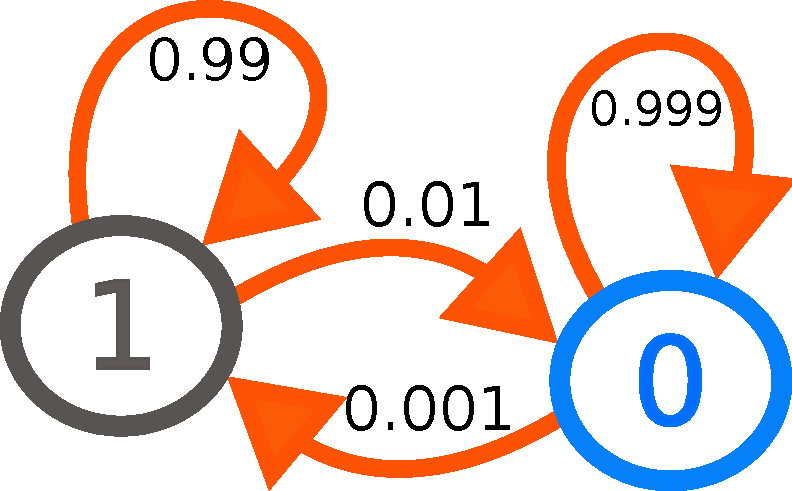
\includegraphics[width=.3\textwidth]{images/markov_chain}
    \caption{Markovova reťaz použitá na generovanie informácie o génoch}
    \label{fig:markov-chain}
\end{figure}

Generovanie robíme pomocou \textit{Markovovej reťaze (Markov Chain)} obr. \ref{fig:markov-chain}. Generujeme podľa aktuálneho stavu a v každom kroku sa podľa pravdepodobnosti rozhodneme či sa prepneme do iného stavu alebo ostaneme v tom istom. Rozhodnutie robíme pomocou \textit{falošnej mince (biased coin)}, kde hlava padne s určitou pravdepodobnosťou, ktorú vopred nastavíme.

%TODO ak bude treba zabrat miesto, tak sem drbnut nejake zdrojaky

Máme vygenerovanú master postupnosť a z nej teraz vyrobíme dve postupnosti pre sekvencie tak, že skopírujeme master sekvenciu, pričom každú 1 s určitou pravdepodobnosťou (v našom prípade $0,1$) zmeníme na 0.

\subsubsection{Simulácia mutácie}

Máme vygenerovanú sekvenciu a ideme vyrobiť zmutovanú sekvenciu. Spravíme to tak, že s určitou pravdepodobnosťou sa nahradí báza z pôvodnej sekvencie inou bázou. Pravdepodobnosť závisí aj od toho, či je na danej pozícii gén v oboch sekvenciách, v jednej, alebo v žiadnej. Na rozhodnutie používame jednu z troch falošných mincí podľa toho, ktorá z možností nastala (tabuľka \ref{tab:mutation-prob}).

\begin{table}[h]
\catcode`\-=12 %kvoli babelu a pomlcke
\centering
\begin{tabular}{lcccc}
Gén A & 0 & 0 & 1 & 1\\
Gén B & 0 & 1 & 0 & 1\\
Pravdepodobnosť & $0,35$ & $0,3$ & $0,3$ & $0,2$\\
\end{tabular}
\caption{Pravdepodobnosti mutácie}
\label{tab:mutation-prob}
\end{table}

\subsubsection{Simulácia delécie}
Deléciu simulujeme opäť pomocou Markovovej reťaze, pretože pri evolúcii majú tendenciu vypadávať súvislé úseky. Pravdepodobnosť, že začneme mazať je $0,01$ a že prestaneme $0,1$.
Ak mažeme, nahradzujeme danú bázu znakom {\verb+'-'+}.

\subsubsection{Využitie}

Simulátor je prvá vec, ktorú sme implementovali a slúžil hlavne na prvotné experimenty.

\todo vieme ho prisposobovat a merat na nom korektnost a uzitocnost modelu, alebo nieco na ten styl

\subsection{Trénovanie modelov}
\todo modeltraining.py

\subsection{Testovanie klasifikátora}
\todo random\_forest\_evaluation.py

\section{Použitie}
\todo v kratkosti o tom ako to vobec spustit so svojimi sekvenciami a modelmi...

\todo mozno sem dat aj moznosti rozsirenia

\todo konfiguracia - constants.py a config.py
